\chapter{Molecular modeling of biological membranes}
\label{chap:methods}

Biological membranes are difficult to study experimentally due to their complex character. 
Among the well established methods for the studies of membranes belong
 NMR                                 \citep{catte16, botan15, seelig80, seelig90, seelig87}, 
small angle x-ray diffraction (SAXD) \citep{ollila16, pabst07}, 
and fluorescence spectroscopy        \citep{javanainen17, melcrova16, vacha09a}. 
Recent advances in cryo-EM             \citep{chiu2017editorial, nogales2015development}
and single-molecule microscopy imaging \citep{ritchie2013single}
reveal another promising tools. 
The resolution of such experimental methods is, however, often insufficient 
for the charactrerization of the structure in atomistic detail. 
In contrast, molecular dynamics simulations provide atomistic resolution of biomolecules.
This makes simulations well suited to be used in conjuction with the experimental methods
bringing deeper insight to the experimentally determined properties. 
In addition, the properties from experiments can be extracted from the simulations 
and compared together, thus cross-validating the two independent approaches. 

%Molecular modeling is one of the newer approaches for studying biological membranes. 
Starting with simple membrane models \citep{Berger97, bockmann04, bockmann03, sachs04, sachs04_potential} 
simulations of membranes have evolved into a field of computational biophysics
that is capable of answering fundamental questions like
how divalent cations modulate the signalling function of \ce{PI(4,5)P_2} \citep{Bilkova2017Calcium}; 
whether there is any preference of calcium cations towards flat plasma membrane or curved synaptic vesicles \citep{magarkar2017};
%whether calcium cations prefer to interact with flat or curved phospholipid bilayers \citep{magarkar2017};
or what are the exchange pathways of plastoquinone and plastoquinol in the photosystem II complex in Thylakoid membranes \citep{eerden17}. 
Recent progress in computational resources and algorithms
has allowed the simulations to grow in spatial scales and composition complexity 
enabling relevant applications in biology. \citep{perspective_cecam_lugano_2018} 


\section{Classical molecular dynamics simulations}
\label{section:md}

In a MD simulation, the system of interest is propagated numerically in discrete time steps using
the Newton equations of motion. 
Interactions between particles, which often represent individual atoms, 
are described by an approximate interaction potential, $U$, also called a \emph{force field}. 
Such a potential can be formally written as a sum of individual terms representing different model interactions.
%The form of the force field varies with the model potentials that are used for the description of the individual interaction components. 
The symbols $K$ are the force constants describing the strengths of the bonded interactions,
which are formally written as
%As an example, the interaction potential of AMBER \citep{ferrer13}, a popular model for biomolecules, has the following form:
 % Amber potential energy form:
\begin{eqnarray}  \label{eq:amber}
  U = & \displaystyle \sum _{bonds} K_b (r-r_{0})^2 + \sum _{angles} K_\Theta (\Theta-\Theta_{0})^2 + \\ \nonumber
      & \displaystyle \sum _{dihedrals} K_n (1+\cos(n\phi -\phi_0)) + \\ \nonumber
      & \displaystyle \sum _{i<j} \left ( s_{ij} ^{VdW} 4 \epsilon _{ij} \left [ \left (\frac{\sigma _{ij}}{r_{ij}} \right )^{12} - \left ( \frac{\sigma _{ij}}{r_{ij}} \right )^6 \right ] + s_{ij}^q \frac{q_i q_j}{\epsilon \, r_{ij}} \right )
\end{eqnarray}
The first three terms represent the intra-molecular forces arising from bond stretching, angle bending, and dihedral angle torsion. 
$r$, $\Theta$ and $\phi$ are their respective dimensions,
and $n$ is the multiplicity of the torsion potential. 

The last terms in the large brackets represent the inter-molecular interactions; 
 Van der Waals and electrostatic forces. 
Depending on the model force field, the non-bonded interactions 
are not evaluated between atoms that are connected by less than three or four bonds, 
which is here formally introduced through the matrix $s_{ij}$ that modifies the interactions accordingly.

%The constants in matrices $\sigma _{ij}$ and $\epsilon _{ij}$  
%respresent respectively the position and the depth of the minimum of the Lennard-Jones potential,
%which is used to model the attractive dispersion interaction 
%and the repulsive forces arising from an unfavourable overlap of electronic shells. 
%$A_{ij}$ and $B_{ij}$ represent the strengths of the attraction and repulsion forces 
%arising from disperion and the overlap of the electronic clouds of the individual particles.  
The interactions representing the 
attractive dispersion and the repulsive excluded volume 
in the empirical interaction potential in Equation~\ref{eq:amber} 
adopt typically the form of Lennard-Jones potential. 
It is expressed in terms of the interaction energy $\epsilon_{ij}$, 
and $\sigma_{ij}$, 
which is the distance,
where the potential crosses zero. 
As the forces at the distances smaller than $\sigma _{ij}$ are strongly repulsive,
these parameters thus also report on the size of the spherical particles
having an impact on the balance of Van der Waals forces with electrostatic forces.


%\todo{Samuli suggested to remove this paragraph.}
%Note that the interactions are simplified not only by the empirical formulae for the individual contributions, 
%but to a large extent also by assuming that the interaction potentials are \emph{pair-wise additive}. 
%Especially in the case of the inter-molecular forces, this is a severe approximation, 
%which neglects the contributions from three and higher-body interactions. 
%It was, however, shown that even such an approximate interaction potential is sufficiently accurate in many cases. \citep{} \todo{Put some application references.} 

The electrostatic interaction creates strong attractive and repulsive forces. 
In classical MD simulation, it is approximated using point partial charges, $q_i$, in the centres of the particles (most often atoms). 
Forces from long distances yield non-negligable contributions,
which must to be accounted for especially in the commonly used 
periodic systems, i.e., in simulations with periodic boundary conditions. 
In neutral systems, this is efficiently done by using the Ewald summation,
in which the long range contributions are calculated in Fourier space rather than in real space
using fast algorithms developed for this purpose. \citep{darden93, essman95}
The formally applied dielectric constant of the medium, $\epsilon$,  
is assumed to be 1 in most force fields for biomolecules. 
In a later section~\ref{section:ecc}, we will show how to modify this interaction 
by changing the dielectric constant $\epsilon$ to include the effects of electronic polarization. 


% Examples, models, applications

Molecular dynamics simulations of biological membranes employ empirical particle-based models of molecules
using the interaction potential, often termed force field, from Eq.~\ref{eq:amber}. 
The models are built using classical non-polarizable particles, 
each representing an individual atom (atomistic models), 
or a group of atoms (united-atom or coarse-grained models). 
The following classical models are among the most popular in membrane modeling:
\begin{itemize}
 \item Atomistic
 \begin{itemize}
   \item CHARMM \citep{klauda10}
   \item Slipids \citep{jambeck12, jambeck12b}
   \item OPLS lipids by \citet{maciejewski14}
   \item Lipid14 \citep{dickson14}
  \end{itemize}

 \item United-atom models
  \begin{itemize}
   \item Berger \citep{Berger97}
   \item CHARMM-UA \citep{lee14}
  \end{itemize}
 \item Coarse-grained
 \begin{itemize}
   \item MARTINI \citep{marrink07}
  \end{itemize}
\end{itemize}

Despite all successes and valuable insights that simulations have provided, 
there is still a large room for possible improvements of the current simulation models. 
For example, recent studies by \citet{botan15, catte16} have shown 
that both structures and interactions of phospholipid models require further optimization 
in order to become capable of interpreting solid state NMR experiments. 
In particular, we have discovered that 
the lack of electronic polarizability is a major issue in any of the models 
from the above mentioned studies %\citep{botan15, catte16}
when interactions with charged moieties become important. \citep{melcr18}
Several possible ways for including polarizability into simulations, both explicit and implicit, 
will be introduced in the following sections. 





\section{Electronic continuum correction as implicit treatment of electronic polarizability}
\label{section:ecc}

The lack of electronic polarizability in classical MD simulations
has been considered a serious issue since the early days of the modeling of lipid bilayers. 
% the commented text on polarizability in this section comes from \citep{huang2017mapping}
There exist two main approaches for the explicit representation of electronic polarizability -- atomic induced dipoles and Drude oscillators.
%The AMOEBA FF adopts the point induced dipole model in which each atom carries an induced dipole moment determined by the electric field and its atomic polarizability. 
%Permanent dipole and quadrupoles are also assigned to each atomic site for a more accurate description of electrostatic interactions. 
The induced dipole approach models the polarizability through a point dipole moment on each atom.
Such an electric dipole is induced by the acting electric field proportionally to its polarizability. 
This model is implemented in the widely adopted force field AMOEBA \citep{amoeba06, amoeba10, amoeba13}.

%The Drude FF adopts the classical Drude oscillator model where auxiliary charges (Drude oscillators or particles) are attached to non-hydrogen atoms with harmonic springs, and the displacement of the Drude particle relative to its parent atom represents the response to the external electric field. 
%Virtual particles representative of lone pairs are included in the Drude FF to improve the treatment of electrostatic interactions typically involving hydrogen bond acceptors.
%The charge distribution between a Drude particle and its parent atom is a finite difference representation of a dipole moment. 
%Similarly, lone pairs can be considered as real space representations of permanent multipoles. 
%Such analogy between the classical Drude oscillator model and the multipole and induced dipole (MPID) model suggests that in theory one can interconvert polarizable FFs between the two models. 
The classical Drude oscillator model is inspired by a classical representation of a lone pair of electrons. 
It uses an auxiliary charge,
also termed Drude oscillator or Drude particle, 
which is attached to each atom through a harmonic spring.
The displacement of the Drude particle respresents the induced polarization proportionally to the acting electric field,
as implemented for example in the Drude force field \citep{lemkul2016empirical}. 

%In this work, we convert the Drude polarizable force field from its original classical Drude oscillator formalism onto a permanent multipole and induced dipole formalism, which we refer to as MPID. 
%We show that a direct mapping without any reparametrization can transfer the Drude FF into the MPID FF, yielding a similar level of agreement as the Drude FF in reproducing condensed phase properties of organic liquids, crystals, and interfaces. 
%Our results thus also serve as an additional validation of these novel simulation algorithms.
Although the two approaches, 
the induced dipole model and the classical Drude oscillator model, 
are very different in how they represent polarizability in simulations,
it was shown that the classical Drude oscillator formalism can be converted to the induced dipole formalism 
proving the two methods to be equivalent. \citep{huang2017mapping}
From the point of view of lipids, however, the classical models with fixed charges and no explicit polarizability that are currently available 
provide comparable accuracy at a fraction of the computational cost of the models with explicit polarization. \citep{lucas12,chowdhary13} 

%The effects of polarization from rather computationally demanding simulations with explicit models 
%can be implemented using an implicit model of polarization. 
Instead of the computationally demanding explicit polarization approach, 
electronic polarization can also be accounted for implicitly.
Such an implicit mean field model of electronic polarizability 
%was developed by \citet{leontyev09} under the name Molecular Dynamics in Electronic Continuum, MDEC. 
termed Electronic continuum correction (ECC) 
was first suggested by \citet{leontyev09}, 
and was then systematically applied to solutions of ions by \citet{Pluharova2014, kohagen14, kohagen16, martinek17}. 
Through a comparison of neutron scattering and/or \emph{ab-initio} molecular dynamics data with classical MD simulations, 
the authors developed an array of models for cations and anions, termed here as ECC-ions,
which provide realistic structures even for concentrated solutions of both monovalent and divalent cations. 
%The term Electronic continuum correction, ECC, originates in the works by \citet{Pluharova2014, kohagen14, kohagen16, martinek17},
%where the rigorously developed theory by \citet{leontyev14} was systematicaly applied to solutions of ions.
%that use ECC to represent electronic polarizability. 

%Electronic continuum correction (ECC) 
In ECC, a system of polarizable particles is represented 
with an equivalent system of particles with fixed charges. %\citep{leontyev09, leontyev10, leontyev11, leontyev14}
%including the effects of electronic polarization \emph{implicitly} in a mean-field way. 
This can be done by a simple transform of the partial charges,
which does not change the form of the empirical force field in Equation~\ref{eq:amber}, 
providing the effects of the electronic polarization in a mean field way at no additional computational cost. 
Although this is technically similar to the phenomenological scaling of partial charges 
applied in earlier studies of aqueous solutions or ionic liquids \citep{jonsson86,egberts94,beichel14},
%where also other possible effects (e.g. charge transfer) were considered,
ECC is a physically well justified and rigorously derived model \citep{leontyev09, leontyev10, leontyev11, leontyev14}.
Assuming that the electronic polarizability of electrons is approximately constant in biological solutions, 
it was shown by \citet{leontyev11} that the electrostatic interactions between atoms 
are screened like in a dielectric continuum 
with an electronic dielectric constant, $\epsilon _{el}$, 
also known as the high frequency dielectric constant. 
This can be formally written as
\begin{equation}  \label{eq:coulomb}
   %U = \frac{1}{2} \displaystyle \sum ^N _{j\neq i} \frac{q_i q_j}{r_{ij}} + \frac{1}{2} \displaystyle \sum ^N _{i,j=1} U ^{dip} _{ij} - \displaystyle \sum ^N _{i=1} E^q(r_i) d_i  \propto  \frac{1}{2} \displaystyle \sum ^N _{j\neq i} \frac{q_i q_j}{\epsilon_{el} \, r_{ij}}  =  \frac{1}{2} \displaystyle \sum ^N _{j\neq i} \frac{q^{ECC}_i q^{ECC}_j}{r_{ij}} 
   %U = \frac{1}{2} \displaystyle \sum ^N _{j\neq i} \frac{q_i q_j}{r_{ij}} + \frac{1}{2} \displaystyle \sum ^N _{i,j=1} U ^{dip-dip} _{ij} - \displaystyle \sum ^N _{i=1} U^{q-dip}_i  \propto  \frac{1}{2} \displaystyle \sum ^N _{j\neq i} \frac{q_i q_j}{\epsilon_{el} \, r_{ij}}  =  \frac{1}{2} \displaystyle \sum ^N _{j\neq i} \frac{\frac{q_i}{\sqrt{\epsilon _{el}}} \frac{q_j}{\sqrt{\epsilon _{el}}}}{r_{ij}}  , 
   U = \frac{1}{2} \displaystyle \sum ^N _{j\neq i} \frac{q_i q_j}{\epsilon_{el} \, r_{ij}}  =  \frac{1}{2} \displaystyle \sum ^N _{j\neq i} \frac{\frac{q_i}{\sqrt{\epsilon _{el}}} \frac{q_j}{\sqrt{\epsilon _{el}}}}{r_{ij}}  , 
\end{equation} 
where $q_i$ is the point charge of the particle $i$,
and $r_{ij}$ are the distances between particles $i$ and $j$.
%$U^{dip-dip} _{ij}$ represent the interactions between induced dipoles and their polarization energies,
%and the terms $U^{q-dip} _i$ are the interactions between point charges and induced dipoles. 
It naturally follows from the above equation that 
embedding all atoms into a dielectric continuum 
is equivalent to a fromal scaling of the atomic point charges 
\begin{equation}  \label{eq:scaling}
 q_i ^{ECC} = \frac{q_i}{\sqrt{\epsilon _{el}}} ,
\end{equation} 
where $q_i$ and $q_i^{ECC}$ are respectively the original partial charges and the scaled charges, 
which represent the effects of the electronic polarization. 
Given that the  high frequency dielectric constant of water is 1.78 (i.e., the square of the refraction index of 1.33), 
the scaling factor for ions in water is $\approx 0.75$. 

It is important to note that the value of the high frequency dielectric constant  
is around 2 for almost any biologically relevant environment \citep{leontyev11}. 
This means that even interfaces like biological membranes do not contain discontinuities of the electronic continuum. 
The dielectric discontinuity in a lipid bilayer thus arises only 
from the orientational polarization of the molecules, which is accounted for explicitly in standard MD simulations.  
Therefore, the same correction for the electronic polarizability can be  
applied throughout the lipid bilayer/aqueous solution interface. 




 

 
 



\section{Implicitly polarizable classical MD models of lipids using ECC}
\label{section:ecc-lipids}

%Simulations with explicitly polarizable models are not frequently used in practice in biophysics. 
%The models employing ECC, however, are on the same level of comupational demands with classical non-polarizable models with fixed charges, yet they implicitly incorporate electronic polarization. 
%The ECC theory was introduced in the above section~\ref{section:ecc}.
%In this section, I will demostrate the application of the ECC theory on phospholipids, 
%where the effects of polarization yield crucial consequences in the accuracy of the description of the interaction with ions. 

%\todo{Describe motivation, goal (cation binding), strategy (ECC). With cation binding, mention it very briefly and point to the next chapter.}
%The structures of the head group region of neutral POPC bilayers from simulations are generally not in agreement with experiments. \citep{botan15}
Simulation studies have revealed that the interactions of phospholipds with cations, especially with divalent cations, 
are overestimated in all classical MD models. \citep{catte16,nmrlipids_proj4}
The neglect of polarizability in the simulations was one of the possible explanations for the observed discrepancy between simulations and experiments. 
Motivated by the accuracy and simplicity of the electronic continuum correction (ECC) applied on ions by \citep{martinek17},
we developed implicitly polarizable models of phospholipids using a similar strategy. 
The newly depeloped model provides accurate interactions between phospholipid bilayers and cations in agreement with experiments, 
which is presented in the next chapter.  
In this section, we show how the model captures the structure of phospholipid bilayers without ions, or with only counterions. 

We chose phosphatidylcholine (PC), phosphatidylethanolamine (PE), and phosphatidylserine (PS)
as representatives of the most common neutral and negatively charged lipids in the plasma membrane \citep{kroon2011_lipid_map, marsh13}. 
The Lipid14~\citep{dickson14} model used for POPE and POPC,
and the Lipid17~\citep{lipid17-future} model, already available from AmberTools \citep{ferrer13},
were used as the starting point for embedding ECC.
It was shown by \citet{botan15, catte16} that such a family of lipid models provides one of the most 
realistic descriptions of the head group order parameters of POPC and their response to ions 
when compared to other available lipid models. 

In case of charged molecules, 
embedding ECC through a linear transformation of the partial charges in Eq.~\ref{eq:scaling} is straightforward -- 
applying ECC to a molecule with a formal charge -1 scales its total charge to $-0.75$. 
Note that the same scaling factor derived from the electronic dielectric constant of water 
was also applied to the charges of ECC-ions by \citet{Pluharova2014, kohagen14, kohagen16, martinek17}.

While the scaling factor of $0.75$ is clearly justified for molecules with a non-zero total charge like ions or POPS,
it is not \emph{a priori} clear what factor shall be used for neutral or zwitterionic molecules, e.g. for POPE, and POPC. 
Unlike the total charge, the partial charges of particles forming molecules in simulations are not physical observables. 
There is a variety of schemes for assigning partial charges to particles in molecules~\citep{Hu2007}. 
The restrained electrostatic potential method (RESP) is, however, the most common method used in biomolecules~\citep{RESP_paper, Singh1984, dickson14}. 
In practice, it is common that water molecules are included in the RESP calculations, 
and charges are subsequently refined to improve certain experimental observables. 
Although such tweaks do not affect the zero total charge for neutral molecules,
it naturally follows from this fitting procedure that the effects of electronic polarizability 
may to some extent be present even in standard force fields~\citep{RESP_paper, Singh1984, jorgensen96, ipolq2013, benavides17}. 
We thus conclude that the scaling factor for partial charges in existing models of neutral molecules does not necessarily need to follow the relation \ref{eq:scaling}.
It is expected instead, that the scaling factor may adopt a slightly higher value than 0.75. 

The ECC correction was applied on top of the Lipid14/Lipid17 models of POPC, POPE, and POPS
by scaling the partial charges of all atoms except for the acyl tails, 
i.e., the polar parts in phospholipids, head group, glycerol backbone, and carbonyl regions. 
Such a choice was guided by the observed strength of interaction with cations. 
In contrast to the head group and the glycerol backbone atoms, 
the acyl chains do not come in direct contact with ions from the solution, 
and they are already highly optimized to provide a good description of the
hydrophobic part of lipid bilayers \cite{dickson14, ollila16, Pluhackova2016}.
In contrast to the acyl tails, the glycerol backbone and the head group regions of phospholipids 
require improvements in any available lipid model~\cite{botan15,nmrlipids_proj4}.

We found that the optimal value for the scaling factor of partial charges of neutral molecules from Lipid14 
that yields accurate responses of the lipid head groups to the charges bound to the membrane
is $0.8$, which is indeed slighly higher than 0.75, 
i.e., the scaling factor for the ions in water. 
This value was found by comparing the results from the simulations with POPC to the experimental 
NMR data on the head group order parameter response to the bound charge. \citep{akutsu81,altenbach84,scherer89}
% Pavel: following sentences seem redundant.
%Note that common empirical scaling factors for solutions of monovalent ions in water 
%are 0.8 or even higher \citep{benavides17,skinner14,nacleps}.  
%In contrast, modern force fields for ionic liquids often employ values around 0.6--0.65, 
%which are on the other hand much lower than $\epsilon^{-1/2}_{el}$ \citep{holm14}.

Although scaling of partial charges improved 
the head group order parameter response and ion binding affinity,
it has at the same time deteriorated certain membrane properties; 
namely the area per lipid generally decreased, often below the experimental values. 
The decrease of the area per lipid is observed to arise from a reduced hydration of the lipid head group region
as the polarity of the head group has decreased in overall after scaling of the charges. 

We compensated for this artifact
by reducing the effective radii of atoms with the scaled charges.
This was explicitly done for POPC by changing the parameters $\sigma$ in the Lennard-Jones potential 
in a similar way as was done previously for the ECC-ions in solution \citep{kohagen14,kohagen16,Pluharova2014}.
Reducing the $\sigma$ parameters of the affected atoms by a factor of $f_\sigma = 0.89$
restored the area per molecule to a value very close to experiment (Table~\ref{tab:apls}). 
Such optimized parameters $\sigma$ were then used for all ECC-lipids, i.e. also for ECC-POPE and ECC-POPS. 
In addition, the X-ray scattering form factors of POPC, POPE and POPS from simulations remained in a good agreement or even improved with these modifications 
(see Figs.~\ref{fig:simVSexpNOions}, \ref{simVSexpNOions_POPE} and \ref{simVSexpNOions_POPS}). 








\subsection{Structural parameters of model membranes with ECC-lipids: Agreement with experiments} 
 
%%%%%%%%%%%%%%%%%%%%%%%%%%%%%%%%%%%%%%%%%%%%%%%%%%%%%%%%%%%%%%
% problemgsolved: NO line breaks in the caption!
\begin{figure}[tb!] 
  \centering 
  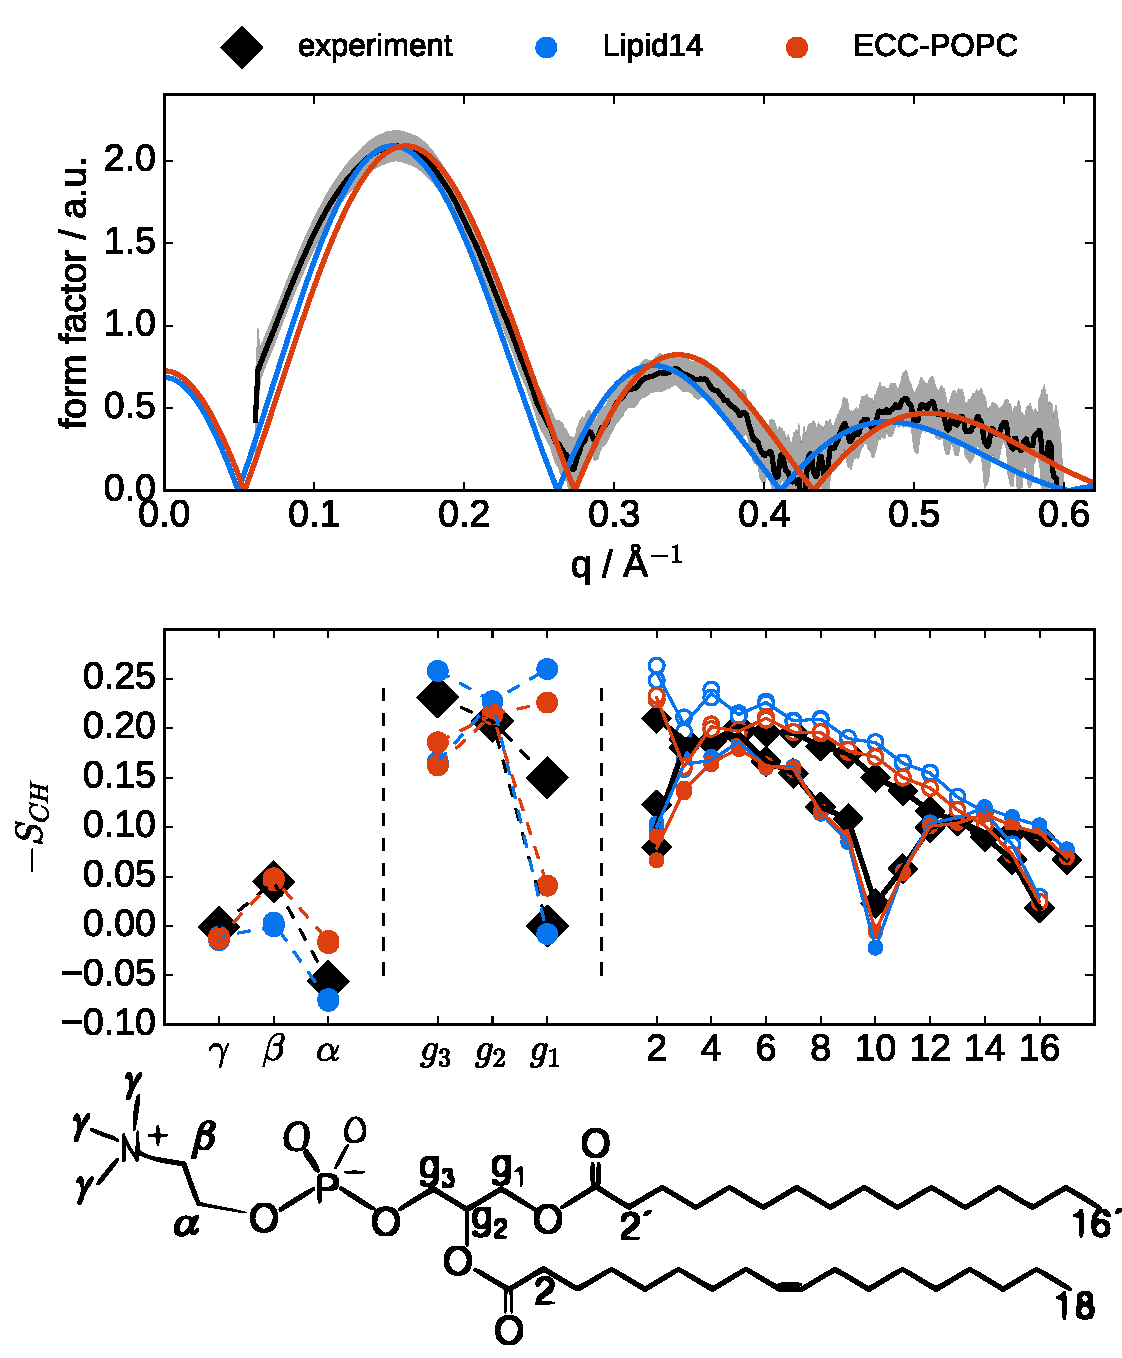
\includegraphics[width=\figwidth]{../img/ecc_popc/Order-parameters_form-factors_exp-L14-ECCL17_q80_sig89_POPC-struct.pdf} 
  \caption{ \label{fig:simVSexpNOions} 
    Top: X-ray scattering form factors from simulations with the Lipid14 \citep{dickson14} and 
    the ECC-POPC \citep{melcr18} models compared with experiments~\citep{kucerka11} at 303~K. 
    Middle: Order parameters of POPC head group, glycerol backbone and acyl chains  
    from simulations with the Lipid14 and the ECC-POPC models 
    compared with experiments \citep{ferreira13} at 300~K. 
    The size of the markers for the head group order parameters correspond to 
    the error estimate $\pm 0.02$ for experiments \citep{botan15,ollila16}, 
    while the error estimate for simulations is $\pm 0.005$
    (Bayesian estimate of 95\% confidence interval \citep{scipy}).
    The size of the points for acyl chains are decreased by a factor of 3 to improve the clarity of the plot.
    Open/closed symbols are used for palmitoyl/oleoyl chains of POPC. 
    Bottom: The chemical structure of POPC and the labeling of the carbon segments. 
  }  
\end{figure} 


\begin{figure}[tb!] 
  \centering 
  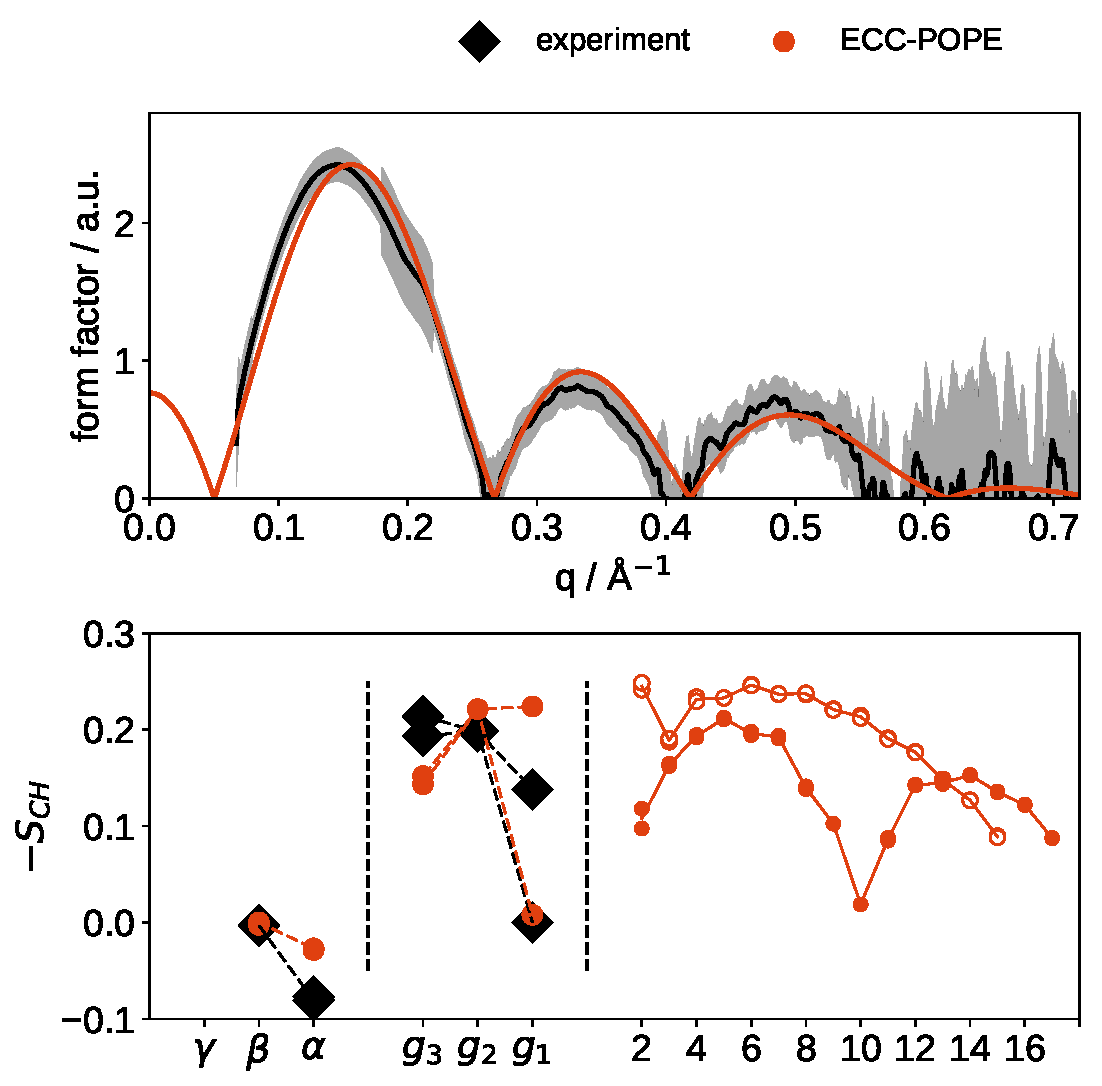
\includegraphics[width=\figwidth]{../img/ecc_pope/Order-parameters_form-factors_exp-ECC-POPE.pdf}
  \caption{\label{simVSexpNOions_POPE} 
    Top: X-ray scattering form factors from simulations with 
    the ECC-lipids model of POPE compared with experiments~\cite{kucerka11} at 313~K. 
    Bottom: Order parameters of POPE head group, glycerol backbone and acyl chains  
    from simulations with the ECC-lipids model of POPE
    compared with experiments by \citet{gally81} (order parameters of glycerol backbone, labeled \emph{E. coli} membrane at~310\,K, ) 
    and by \citet{seelig76, seelig80} (order parameters $\alpha$ and $\beta$ from DPPE at~341\,K).
    The signs of the order parameters were not determined in the experimnets, same signs as in POPC (Fig.~\ref{fig:simVSexpNOions}) are assumed. 
    Open/closed symbols are used for palmitoyl/oleoyl chains of POPE. 
    The chemical structure of POPE is the same as for POPC in Fig.~\ref{fig:simVSexpNOions}, 
    but the methyl groups in choline (denoted with $\gamma$), which are substituted with hydrogen atoms in PE. 
  }  
\end{figure} 


\begin{figure}[tb!] 
  \centering 
  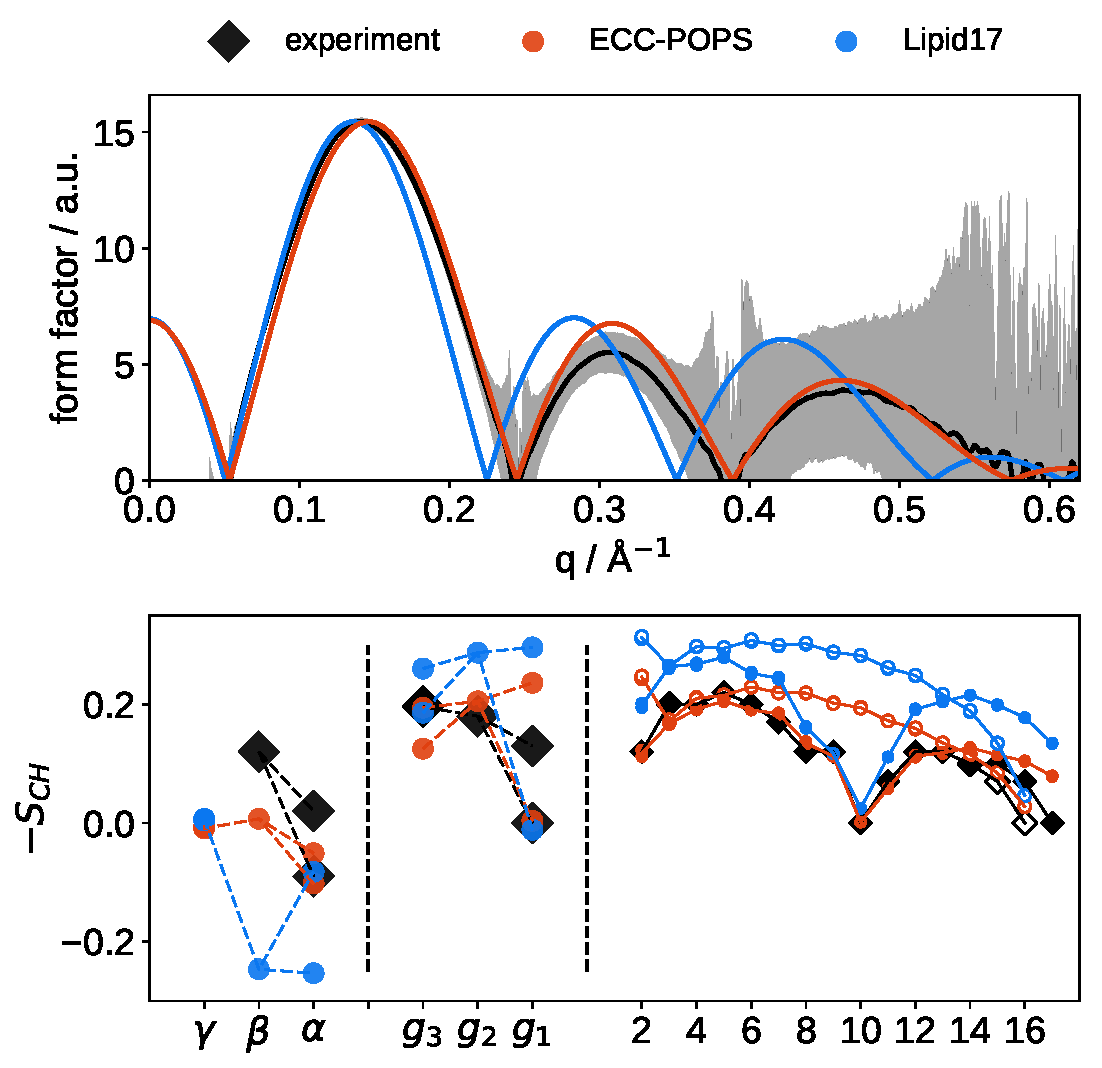
\includegraphics[width=\figwidth]{../img/ecc_pops/Order-parameters_form-factors_exp-L17-ECC-lipids.pdf}
  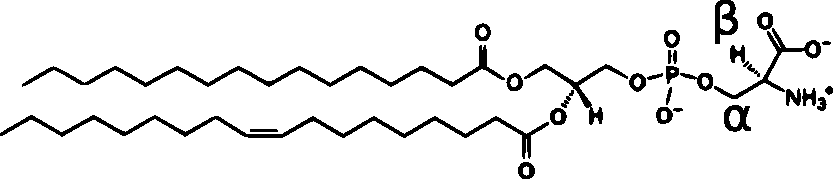
\includegraphics[width=\figwidth]{../img/ecc_pops/pops_chemfig.pdf} 
\hfill
  \caption{\label{simVSexpNOions_POPS} 
    Top: X-ray scattering form factors from simulations with the Lipid17 \citep{lipid17-future} and 
    the ECC-POPS models compared with experiments~\citep{kucerka14} at 298~K. 
    Middle: Order parameters of POPS head group, glycerol backbone and acyl chains  
    from simulations with the Lipid17 \citep{lipid17-future} and the ECC-POPS models 
    compared with experiments at 298~K. \citep{nmrlipids_proj4}
    Open/closed symbols are used for palmitoyl/oleoyl chains of POPS. 
    Bottom: The chemical structure of POPS and the labeling of the carbon segments. 
  }  
\end{figure} 
%%%%%%%%%%%%%%%%%%%%%%%%%%%%%%%%%%%%%%%%%%%%%%%%%%%%%%%%%%%%%%
 
\begin{table}[tb!] 
\centering
  \caption{Values of the area per lipid (APL) of POPC, POPE and POPS bilayers 
           at temperatures $T$ without additional ions. \label{tab:apls} } 
  \begin{tabular}{l|c c} 
    \multicolumn{3}{c}{POPC} \\
    model          & APL / Å$^2$   & $T$ / K  \\ 
    \hline 
    Lipid14 POPC \citep{melcr18}    & 65.1$\pm$ 0.6  &  300 \\ 
    Lipid14 POPC \citep{dickson14}  & 65.6$\pm$ 0.5  &  303 \\ 
    \hline 
    ECC-POPC     \citep{melcr18}    & 63.2$\pm$ 0.6  &  300       \\ 
    \hline 
    experiment (SDP model) \citep{kucerka11} & 64.3  &  303    \\ 
    \hline 
    \multicolumn{3}{c}{} \\
    \multicolumn{3}{c}{POPE} \\
    model          & APL / Å$^2$   & $T$ / K  \\ 
    \hline 
    ECC-POPE                 & 56.7$\pm$ 0.8  &  298 \\ 
    \hline 
    experiment   \citep{parsegian89} & 56.6  &  310    \\ 
    experiment   \citep{rappolt03}   & 59--61 &  303--313  \\ 
    \hline 
    \multicolumn{3}{c}{} \\
    \multicolumn{3}{c}{POPS} \\
    model          & APL / Å$^2$   & $T$ / K  \\ 
    \hline 
    Lipid17 POPS              & 53.5$\pm$ 0.8  &  298 \\ 
    \hline 
    ECC-POPS                & 60.3$\pm$ 0.6  &  298       \\ 
    \hline 
    experiment (SDP model) \citep{kucerka14} & 62.3  &  298    \\ 
    \hline 
  \end{tabular} 
\end{table} 
 
 
We compared X-ray scattering form factors and NMR order parameters of bilayers
in pure water without any ions (or only counter ions)
from simulations and experiments
as the first step in the assessment of the quality of the model. 
The experimental X-ray scattering form factors 
of a bilayer are well reproduced for all lipids employing the presented ECC-lipids model 
(see Figs.~\ref{fig:simVSexpNOions}, \ref{simVSexpNOions_POPE} and \ref{simVSexpNOions_POPS}). 

The area per lipid is often used as a relatively simple structural parameter reporting on the bilayer properties and the packing of lipids. 
In experiments, modeling is used on top of the scattering factors to obtain it \citep{kucerka14}. 
From simulations, this property is easily extracted. 
We compare the values from experiments and simulations in Table~\ref{tab:apls}. 

The area per lipid of POPC in simulation with ECC-lipids model is smaller by $\approx 1Å^2$ 
than the experimental value derived from the SDP model \citep{kucerka14}. 
The values of the area per lipid of the ECC-POPC model vary slightly 
when simulated with different water models, however,
they are still close to the experiment. \citep{melcr18}


The experiments with POPE bilayers were performed only at higher temperatures than in the simulation \citep{parsegian89, rappolt03},
however, if we extrapolate the experimental values using the series in the work by \citet{rappolt03} 
(i.e., change of $\approx 1Å^2$ for each $5^\circ$C), 
the extrapolated estimate of the area per lipid from the simulation 
lays between the two distinct values from the experiments in Table~\ref{tab:apls}. 


While the agreement between the scattering form factors 
from the simulation of a pure POPS bilayer and experiment 
are excellent (Fig.~\ref{simVSexpNOions_POPS}),
there is a non-negligable difference between the values of the area per lipid in Table~\ref{tab:apls}. 
Since both values are derived from the scattering form factors through modeling of the electron density of the bilayer,
we cannot decide, which of the values is more reliable. 
In general, we can conclude that ECC-lipids
%the presented lipid models with ECC-lipids 
reproduce the experimental structural parameters of the lipid bilayers 
with a comparable accuracy to existing state-of-the-art lipid models~\citep{botan15, ollila16, Pluhackova2016}. 
 
The head group and acyl chain order parameters within ECC-lipids
are in general in a good agreement with the experimental values 
as shown in Figs.~\ref{fig:simVSexpNOions}, \ref{simVSexpNOions_POPE},  and \ref{simVSexpNOions_POPS}. 
The acyl chain order parameters in particular are almost all within the experimental error bars.
The order parameters of the head groups are at an accuracy comparable to 
other currently available classical models of lipids \citep{botan15, catte16, Pluhackova2016}. 

The head group order parameters $\alpha$ and $\beta$ are highly relevant for this work,
as they are being used in the electrometer concept (introduced in section~\ref{section:electrometer}). 
For POPC in pure water, the order parameter $\beta$ agrees well with the experiment, 
while the order parameter $\alpha$ is somewhat lower. 
In the case of POPS, the situation is a bit more complicated
compared to POPC as the order parameter $\alpha$ exhibits a notable forking (see Fig.~\ref{simVSexpNOions_POPS}).
One of the order parameters of ECC-POPS, $\alpha_1$, agrees well with the experiment, 
while the other, $\alpha_2$, adopts a higher value underestimating the experimentally reported forking. 
There is only one order parameter $\beta$ in POPS, 
which has a higher value closer to zero in the ECC-lipids model than in experiment. 
Such a feature suggests that the model overestimates the orientational freedom of its head group. 

To our knoweldge, there are no data on the order parameters in POPE. 
To get at least a rough estimate of the structure of PE head group from experiments, 
we can compare to either DPPE, which has palmitoyls in both acyl tails, and is measured at a different temperatrue~341\,K \citep{seelig76, seelig80};
or a mixture of PE lipids from the membrane of \emph{E. coli} at~310\,K, \citep{gally81}. 
Such data are used in Fig.~\ref{simVSexpNOions_POPE} to provide estimates of the order parameters for related systems. 
 
 
 






\section{Modeling of transmembrane potential}

The intracellular environment of cells contains a weak electrolytic solution of \ce{KCl}, 
while there is a similarly weak solution of \ce{NaCl} on the extracellular side. 
The concentrations of these salts, usually around 150\,mM, 
are regulated and maintained out of equilibrium through specific channels and pumps 
to provide cellular functions and general homeostasis conditions \citep{Bezanilla2008, Knudsen_book2002}. 
The unequal distribution of ions on either side of the membrane
gives rise to a transmembrane potential. 
For instance, the concerted action of voltage-gated ion channels and pumps in neurons 
modulates their transmembrane potential
providing a fast signal transduction through the axons \citep{Knudsen_book2002, Storace2015, Sung2015}. 
The common magnitude of the transmembrane potential in cells is in the range of 10--100~mV. 
In experiment, the membrane potential can be measured using the patch clamp technique \citep{Bezanilla2008}
and the more modern voltage-sensitive fluorescent probes \citep{Storace2015, Sung2015}. 

The transmembrane potential in simulations can be modeled by several methods. \citep{Tieleman2001,Sin2015, Roux1997, sachs04_potential}.
In particular, 
there are two approaches for the modeling of 
the membrane potential in atomistic molecular dynamics simulations --
 the constant electric field method \citep{Roux1997,Roux2008,gumbart_constant_2012}, 
and
 the ion-imbalance method \citep{sachs04_potential,Delemotte2008}. 
Both of these methods have been successfully used to study membrane electroporation or voltage-sensitive proteins \citep{Vargas2012, bockmann_kinetics_2008, gumbart_constant_2012, kutzner_computational_2011, casciola_molecular_2014}. 
These two practically independent developments were compared and connected together in our work \citep{melcr16},
where we prove them to be equivalent models of the transmembrane potential yielding indistinguishable results, 
at least for electrolytes formed by the same monovalent ions on both sides of the membrane. 
We used simulations 
in which we simultaneously applied both methods
with the same magnitude but opposite polarity 
yielding zero transmembrane voltage in total 
to highlight possible artifacts. 
The comparison in Fig.~\ref{fig:potentialKCl} shows 
that such a setup is indistinguishable 
from simulations without voltage within the achievable accuracy. 
The electric field induced by the voltage 
exists exclusively in the hydrophobic region of the membrane,
where it has an almost constant strength. 
This finding provides clues to understanding the evolutionary design of volage-gated proteins. \citep{Vargas2012} 
Moreover,
the structure of the bilayer is preserved even at high voltages at the time scales of our simulations,
unlike that of water at the interface with the hydrophobic core of the bilayer
underlining its importance in electroporation. \citep{bu2017mechanics}

\begin{figure}[btp]
\begin{center}
\includegraphics[width = \figwidthfull]{../img/pot+field+chargedens_6plot_KCl-page001.png}
 \caption{The transmembrane potential (A,B), the electric field intensity (C,D), and the charge density (E,F) profiles for simulations of a POPC bilayer with 150\,mM concentration of \ce{KCl}. 
ZERO stands for simulations without any applied voltage,
IIMB stands for the ion imbalance method,
CEF  stands for the constant electric field method,
and FxI denotes the special setup, in which the two methods are applied simultaneously. 
The gray area shows the standard error. 
The voltage drop across the membrane is $499\,$mV for IIMB and $486\,$mV for CEF with the error of about $7\,$mV.  
}
\label{fig:potentialKCl}
\end{center}
\end{figure}

